\chapter{BOBShield}
\label{kap:1}
BOBShield je zariadenie, ktoré vzniklo ako súčasť vačšieho projektu AutomationShield. Predstavuje  nízko nákladový miniaturizovaný systém - Gulička na tyči, ktorý slúži ako učebná pomôcka pri predmetoch zaoberajúcich sa riadením systémov. Zariadenie používa servomotor pre otáčanie trubičkou, v ktorej sa pohybuje gulička. Cieľom experimentu je nastaviť naklonenie trubičky tak aby bolo sa gulička nachádzala v nami požadovanej pozícii alebo aby sledovala nami určenú referenčnú trajektóriu. Zariadenie svojimi malými rozmery a nízkymi nákladmi na výrobu poskytuje možnosť pre študentov vyskúšať si riadenie v praxi mimo zariadení v školských laboratóriách, ktorých dostupnosť výrazne náročnejšia.     
\section{AutomationShield}
\label{kap1.1}
AutomationShield je projekt zameraný na tvorbu jednoduchých a cenovo dostupných zariadení, ktoré slúžia ako učebné pomôcky pri výučbe riadenia systémov. Keďže cieľom je práve dostupnosť pre všetkých, ktorý sa zaujímajú o riadenie a regulovanie systémov, ide o voľne dostupný hardvér a softvér. Základom celého projektu je práve mikropočítač, ktorý na riadenie využívame. Ide o Arduino, taktiež opensource hardvér a softvér, ktorý má medzi študentami pomerne veľkú základňu a je veľmi obľúbenou voľbou pre výučbu mikroprocesorov techniky na  univerzitách a školách technického zamerania. Na tvorbu jednotlivých zariadení sa používajú dosky rozširujúce funkcionalitu samotnej arduino dosky, vo svete všeobecne známe ako „shieldy“. V podstate nejde o nič iné než o dosku plošných spojov (PCB), ktorá sa stará o elektrické spojenie medzi jednotlivými komponentami na zariadení a arduinom Keďže väčšina typov arduino dosiek dodržiava zaužívané rozloženie pinov na doske, nie je používanie shieldov obmedzené len je jednu z nich. Z dôvodu dostupnosti, je podstatnou časťou tohto projektu práve nízka cena výsledného zariadenia. V priemere dosahujú jednotlivé shieldy cenu okolo 20 eur. Ďalšou častou sú práve minimálne rozmery zariadení, čo poskytuje jednoduchú manipuláciu a možnosť využívať ich naozaj kdekoľvek, čo samo o sebe robí tento projekt veľmi sympatickým a pre používateľa vytvára dojem jednoduchosti a prístupnosti.
 
V projekte existuje niekoľko rôznych typov zariadení, ktoré simulujú riadenia rozličných systémov, no či už ide o regulovanie teploty, tlaku alebo pozície telesa v systéme, jedná sa o miniaturizované verzie väčších systémov. Okrem hardvéru je v AutomationShielde vyvíjaný aj softvér pre riadenie týchto systémov. Medzi programy využívané pre tvorbu API - rozhraní pre programovanie aplikácií patrí v základe Arduino IDE, MATLAB a Simulink.  


\section{Experiment - Gulôčka na tyči}
\label{kap:1.2}

 Gulička na tyči – po anglicky Ball on Beam, odkiaľ pochádza aj názov nášho zariadenie, je dynamický systém, ktorý pozostáva z dlhej tyče pripojenej k servomotoru, ktorá sa jeho pôsobením nakláňa a guličky, ktorá sa pohybuje po tyči dopredu a dozadu, v závislosti od jej naklonenia. Ide o veľmi populárny príklad používaný pri výučbe teórie riadenia. Gulička na tyči je teda nestabilný, nelineárny systém s otvorenou slučkou. Aj pri malej výchylke trubičky sa gulička skotúľa do jednej z krajných polôh tyče. Stabilizáciu guličky v určitej pozícii je potrebný riadiaci systém, ktorý meria polohu guličky na tyči  a na základe získaných hodnôt vyhodnocuje nastavenie polohy tyče. Na obrázku \ref{OBRAZOK 1.2} môžeme vidieť parametre systému, kde zmena uhla  $\theta$ pôsobí cez rameno páky na tyč a spôsobí jej otočenia o uhol $\alpha$. Keď sa zmení uhol z horizontálnej pozície, gravitácia zapríčiní pohyb guličky po tyči. Úlohou riadiaceho systému je teda aby sme vedeli ovládať pozíciu guličky.


\begin{figure}[!h]
	\centering
	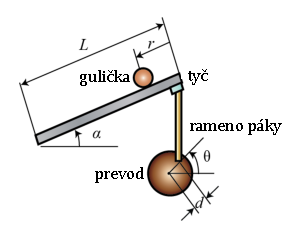
\includegraphics[width=80mm]{obr/experimentBOB.eps}
	\caption{Systém gulička na tyči \cite{BOBexperiment}}\label{OBRAZOK 1.2} 
\end{figure} 


Náš systém sa od systému na obrázku mierne líši. Namieste tyče sa gulička pohybuje uprostred trubičky a jej stred otáčania sa nenachádza na konci trubičky ako to môžeme vidieť na obr. \ref{OBRAZOK 1.2}. Uložená je v držiaku, ktorý sa nachádza v jej strede a práve pomocou neho je na ňu prenášaný krútiaci moment zo servomotora. V pôvodnej verzii sa teda nenachádzal ani prevod spomenutý na obrázku, držiak bol priamo pripevnený k servomotoru. Prevod sme však pri vylepšovaní hardvéru zahrnuli do jeho zmien, no oproti klasickému riešeniu uvedenému na obrázku sme zvolil náš vlastný originálny prístup. Výhodnou tohto spôsobu zostavenia systému sú jeho rozmery, sú dostatočne malé aby sme vedeli celý model uložiť na Arduino shield.


\section{Bobshield R2}
\label{kap:1.3}
Vývoj zariadenia je náročný proces vyžadujúci si určitý čas, skúšanie nových možností a vylepšení, či už sa jedná o hardvérovú alebo softvérovú časť. Používaním zariadenia postupne dochádzame k novým nápadom na vylepšenie a tie postupne implementuje a dolaďujeme, čím sa blížime k ideálnemu riešeniu. Tento stav však takmer nikdy nedosiahneme vzhľadom k neustálemu vývoju a preto je vždy priestor na zmeny a aktualizáciu projektu. Aj BOBShield si už prešiel mnohými zmenami, čo sa použitých komponentov, dizajnu alebo API  týka. Prvá verzia BOBShield R1 (obr.\ref{OBRAZOK 1.3})  vznikla ako výsledok práce študentov na predmete mikroprocesorová technika 2, na ústave Automatizácie a merania STU v Bratislave. 

\begin{figure}[h]
	\centering
	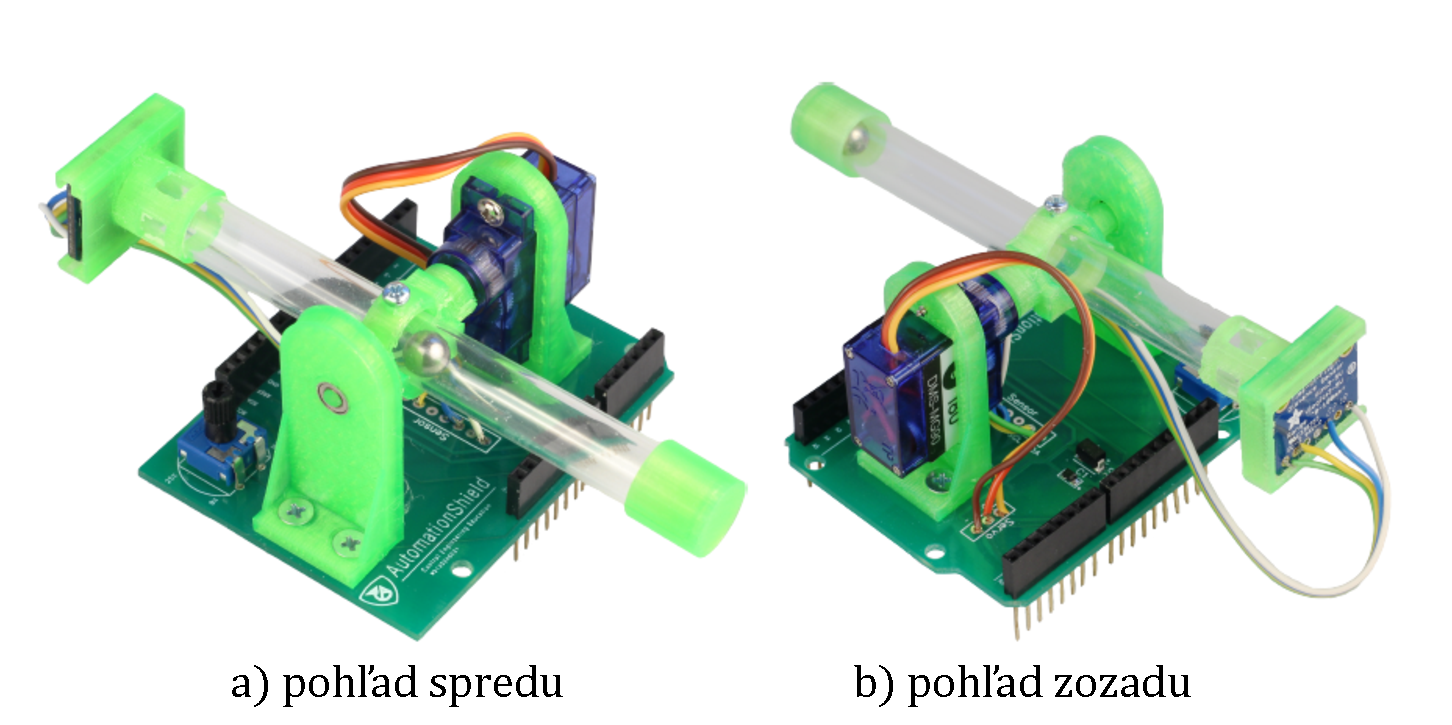
\includegraphics[width=80mm]{obr/R1.eps}
	\caption{BOBShield R1 \cite{Anicka}}\label{OBRAZOK 1.3} 
\end{figure} 

Poslednou verziou je BOBShield R2 (obr. \ref{OBRAZOK 1.4}) a bola vytvorená ako súčasť diplomovej práce na Strojníckej fakulte STU v Bratislave.  Oproti prvej verzii prišlo k zmenám hardvéru, kde bolo zmenené rozloženie komponentov na shielde, došlo k vylepšeniu 3D prvkov a zmene veľkosti trubičky a guličky. Tiež boli vytvorené nové príklady pre zariadenie v protredí Arduino IDE ako napríklad identifikácia systému. 

\begin{figure}[h]
	\centering
	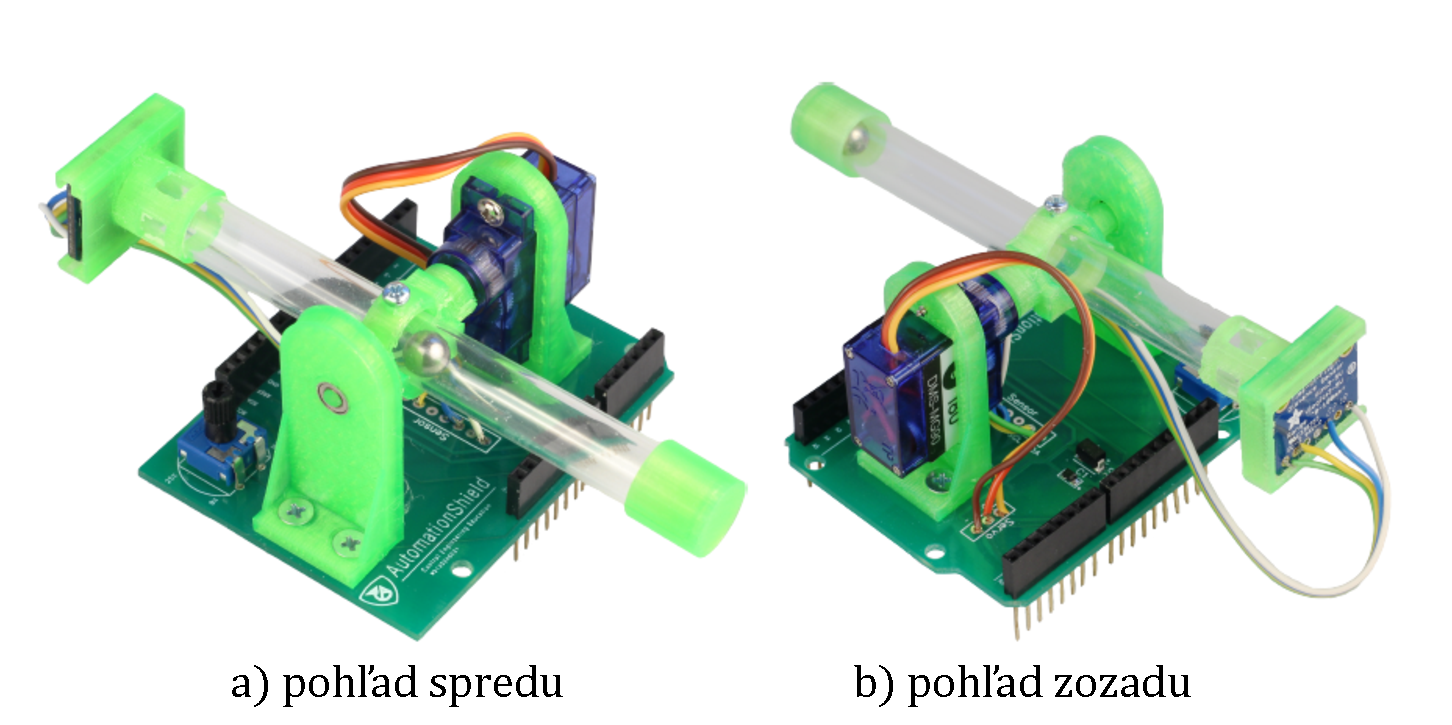
\includegraphics[width=80mm]{obr/R1.eps}
	\caption{BOBShield R2 \cite{Anicka}}\label{OBRAZOK 1.4} 
\end{figure} 

\subsection{R2 softvér}
\label{kap:1.3.1}
Z programových prostredí, ktoré sa v projekte AutomationShield využívajú k riadeniu systému, konkrétne ide o Arduino IDE, MATLAB a Simulink bolo vytvorené API (aplikačné programovacie prostredie) len v prostredí Arduino IDE. Pozostáva z knižnice BOBShield.h a niekoľkých príkladov ako je regulácia alebo identifikácia systému. To ponúka priestor pre tvorbu nových API v už spomenutých programovacích prostrediach. 


\subsection{R2 hardvér}
\label{kap:1.3.2}
Z hľadiska hardvéru ponúka verzia R2 priestor pre analýzu použitých komponentov a ich porovnanie s novými možnosťami ponúkanými na trhu. Tiež je možné zvýšenie presnosti otáčania trubičky o implementáciou už spomínaného prevodu medzi servomotorom a držiakom trubičky. Z toho následne vyplýva aj zmena 3D prvkov a celkového dizajnu zariadenia. 

